\documentclass[11pt]{article}
\usepackage[margin=0.75in]{geometry}
\usepackage{amsmath,amssymb,graphicx,hyperref}
\setlength{\parindent}{0pt}\setlength{\parskip}{4pt}
\setlength{\emergencystretch}{3em}
\begin{document}
{\Large Actual public signed Hankel reconstruction}\par
2026-11-13. Source\path{17fd598fd}. Unsigned evidence [pcc:unverified].

For $|S|=2a$, $a\ge2$, actual distinct abscissas $x\in S$, public branches
$z(x)^2=f(x)$ and $\deg f=3$, define
\[
 G=\prod_{x\in S}(X-x),\quad w_x=\prod_{t\in S\setminus\{x\}}(x-t)^{-1},\qquad
 M_{jk}=\sum_{x\in S}w_xz(x)x^{j+k},\quad 0\le j,k<a-1.
\]
This is an actual public symmetric Hankel matrix. Its dimension is $a-1$;
its entries depend on the branches, without planted norm polynomials
[pcc:unverified].

\textbf{Exact certificate.} Construct $s$ by Lagrange interpolation. For
$\deg B<a-1$, set $A=sB\bmod G$. The finite top-moment test gives
\[
 \deg A\le a\quad\Longleftrightarrow\quad M\operatorname{coeff}(B)=0.
\]
If $\det M=0$, extract a nonzero kernel vector, and use Polynomial.ofFn to
construct $B$ and its degree bound. At every actual node, $A=zB$ and $z^2=f$;
therefore $G\mid A^2-fB^2$. The pole bound caps the norm degree at $2a$.
It cannot vanish: $2\deg A=3+2\deg B$ is impossible for $B\ne0$.
Thus $A^2-fB^2=cG$ with $c\ne0$. The publicInputCertificate theorem supplies
the interpolant itself; no successful $A/B$, inverse, moment or rank oracle
is assumed [pcc:unverified].

\begin{center}
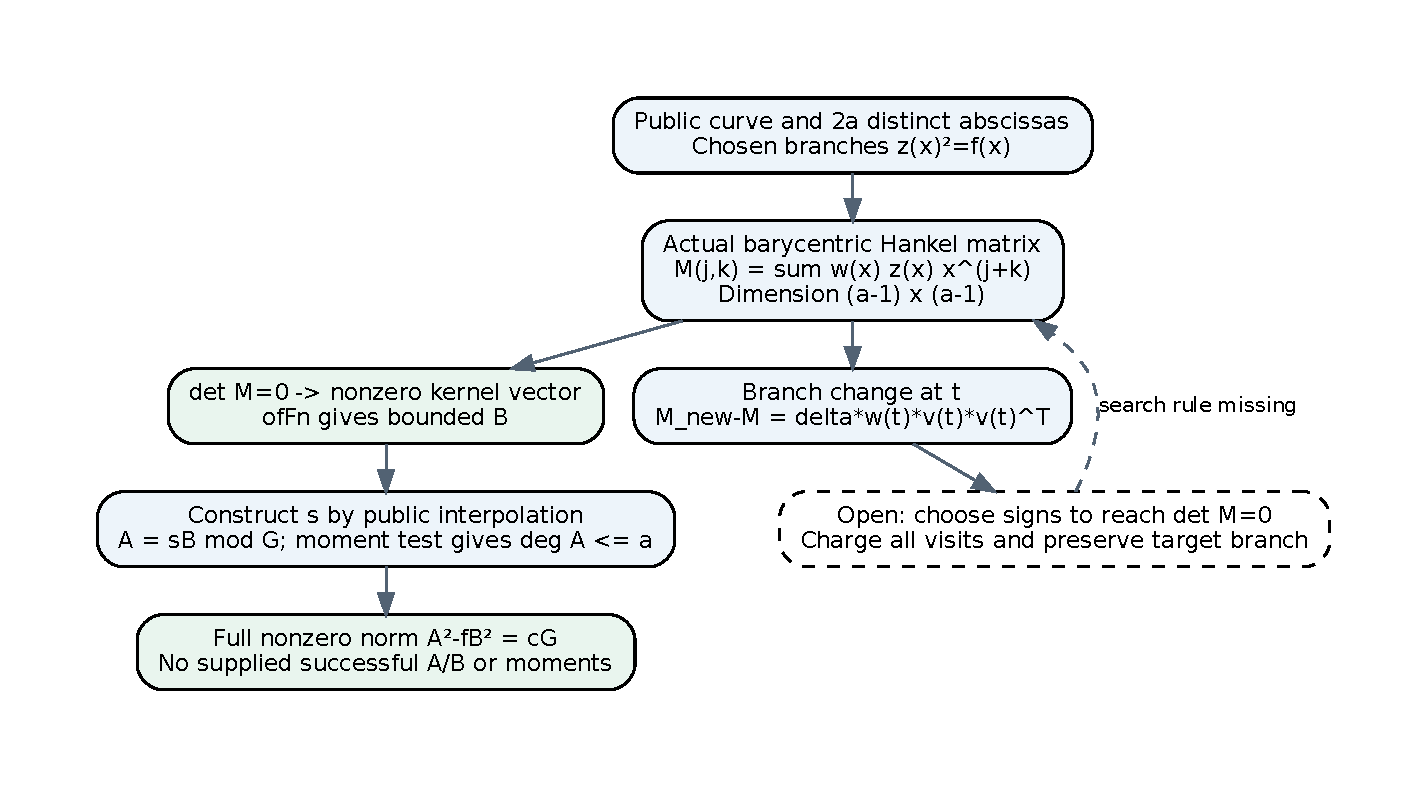
\includegraphics[width=0.94\linewidth,height=0.34\textheight,keepaspectratio]{hankel.pdf}
\end{center}

\textbf{Finite moment proof.} For $\deg R<\deg G$, the moments
$[X^{\deg G-1}](RX^j\bmod G)$, $j<\deg G-a-1$, vanish exactly when
$\deg R\le a$. A forbidden highest coefficient is detected by the complementary
monomial $X^{\deg G-1-\deg R}$. For actual node products, Lagrange's coefficient
formula makes these moments the explicit barycentric sums above
[pcc:unverified].

\textbf{Branch update.} Changing $z(t)$ by $\Delta$ gives
$M_{\rm new}-M=\Delta w_t v_tv_t^T$, $v_t=(1,t,\ldots,t^{a-2})$.
A sign flip has $\Delta=-2z(t)$. Arbitrary continuous corrections must still
satisfy the curve point equations. The earlier $W$-jet family has not been
mapped to this construction [pcc:unverified].

\newpage
{\Large Fixed controls, evidence and remaining search}\par
\textbf{Actual finite matrices.} Over F17, $f=X^3+2X+2$, use
$(0,6),(3,1),(5,1),(6,3),(10,11),(13,7)$. Weights are
$[4,9,15,14,16,10]$ [pcc:unverified].
\begin{center}
\begin{tabular}{lccc}
Supplied branches & Hankel matrix & determinant & kernel dim.\\\hline
Listed points & $\begin{pmatrix}13&15\\15&16\end{pmatrix}$ &0&1\\[6pt]
Only $(13,7)\to(13,10)$ & $\begin{pmatrix}9&14\\14&3\end{pmatrix}$ &1&0
\end{tabular}
\end{center}
The full $6\times6$ and compressed $2\times2$ kernels are checked in both
directions. Positive reconstruction gives $A=[14,2,7,3]$, $B=[8,1]$, $c=9$,
ascending coefficients, checked against original rows, points, degree bounds
and the full norm. No supplied successful $A/B$ enters the solve
[pcc:unverified].

All six branch updates for each assignment are checked entrywise. Independent
Leibniz determinants also check the cofactor update formula on these finite
$2\times2$ cases. Positive single-flip determinants are
$[14,8,16,15,14,1]$. A wrong barycentric weight changes the matrix and rejects
the one returned positive candidate; the empty flipped kernel records zero
candidate checks. These are fixed identity controls, not independent trials,
a sign search or a measured speed comparison [pcc:unverified].

\textbf{Proof/evidence.} Fourteen new statements in NormSignedHankel;
whole-study tracked-source gate245 statements,0 additional trusted axioms.
Builds001/002 fail;003 passes with a warning;004 removes it;005 supplies the
actual public interpolant. A separate fresh replay includes imports; its exact
receipt is in checks.json/fresh-status.json. Native tests002:9 passed;
strict clippy001 fails on an allocation,002 passes after repair. Preserve
all original logs and exits [pcc:unverified].

Public-input claim: \path{PCC-20261113-e1c10e}.\par
Degree equivalence: \path{PCC-20261113-864c3f}.\par
Literal matrix update: \path{PCC-20261113-f1012f}.\par
Original native artifact: \path{PCC-20261113-a6a482}.\par
All remain unsigned; default-PATH source-only checks are not\_covered,
separate from explicit-toolchain kernel checks. Lean4.35.0, CryptoLean
\path{148f5dc389b}, Mathlib\path{cfc55fc58714}; full source hashes,14-statement
proof map, claims and artifact digest are in the source-linked README.

\textbf{Next obligation and complete cost.} Choose the public branch signs
so that this actual matrix is singular, keeping a target branch fixed. A direct
scan still has $2^{D-1}$ assignments; polynomial-cost Hankel algebra changes
no exponent by itself. The required total remains $\exp(o(\log r))$, including
setup, all rejected candidates, divisors and scalar verification. Next test:
constrained branch repair and corank/uniqueness structure, rather than assuming
a rank gradient. No such search advantage is established here [pcc:unverified].

\textbf{Primary sources.} Zeh--Gentner--Augot1110.3898, equation3 and key
 equations: GRS weights/Hankel structure are prior art. Cheng cs/0507026,
sections3/4: worst-case reductions, not an ordinary-curve average-case bound.
Li--Wan--Zhang1501.01138: dense-set and decision assumptions must be charged.
Iwata ISAAC2017: independent pair unions differ from dependent transversals.
Mahalanobis2607.09814v2: fixed-defect success cost is retained. Exact URLs and
read scopes in README. KB tools absent; wrapper exits127. No exhaustive,
priority, global impossibility or new ECDLP algorithm claim.
\end{document}
